\chapter{Methods}

In this chapter, the methods used in this research are explained. First, Coulomb dissociation is introduced as a method to research the halo structure of $^{17}$B. For the part of it, equivalent photon method as a tool for investigating the soft $E1$ excitation of $^{17}$B is described. The $E1$ reduced transition probability $B(E1)$ and the geometrical information which is related to dineutron correlation can be obtained. Next, for extracting the Coulomb dissociation cross section from experimental data, the subtraction of nuclear breakup component is explained. Finally, the invariant mass method for the reconstruction of experimental data is explained. 

\section{Coulomb Dissociation}
\begin{figure}[t]
    \centering
    \setlength{\unitlength}{1mm}
    \begin{picture}(100,52)
        % Boron-17 nucleus
        \put(10,40){\circle{15}}
        \put(10,42){\circle{10}}
        \put(7,41){\footnotesize ${}^{15}$B}
        \put(8,35){\circle*{2}}
        \put(12,35){\circle*{2}}
        \put(8,30){\footnotesize n     n}
        \put(6,49){${}^{17}$B}

        % Arrow to excited state
        \put(20,40){\vector(1,0){20}}

        % Excited Boron-17 nucleus
        \put(50,40){\circle{15}}
        \put(50,42){\circle{10}}
        \put(47,41){\footnotesize ${}^{15}$B}
        \put(48,35){\circle*{2}}
        \put(52,35){\circle*{2}}
        \put(48,30){\footnotesize n      n}
        %\put(50,20){\line(0,-1){12}}
        \put(50,15){\circle{12}}
        \put(48,14){\footnotesize Pb}
        \put(46,49){${}^{17}$B$^*$}

        % Gamma ray
        \multiput(50,21)(0,1){7}{\line(0,1){0.5}}
        \multiput(50,9)(0,-1){7}{\line(0,-1){0.5}}
        \multiput(53,20)(0.4,1){7}{\line(0.4,1){0.2}}
        \multiput(47,20)(-0.4,1){7}{\line(-0.4,1){0.2}}
        \multiput(53,10)(0.4,-1){7}{\line(0.4,-1){0.2}}
        \multiput(47,10)(-0.4,-1){7}{\line(-0.4,-1){0.2}}

        %\multiput(50,15)(-3,3){5}{\line(0,-0.3){1}}
        \put(42,20){\footnotesize $\gamma$}

        % Arrow to final state
        %\put(60,20){\vector(1,0){20}}

        % Final state boron-15
        \put(90,47){\circle{10}}
        \put(87,45.5){\footnotesize ${}^{15}$B}
        \put(60,40){\vector(1,0.3){20}}
        \put(96,49){\footnotesize \( E_{^{15}\text{B}}, \vec{P}_{^{15}\text{B}} \)}

        % Final state neutron 1
        \put(90,33){\circle*{2}}
        \put(86,33.5){\footnotesize $n$}
        \put(60,40){\vector(1,-0.25){25}}
        \put(92,33){\footnotesize \( E_{n1}, \vec{P}_{n1} \)}
        % Final state neutron 2
        \put(90,28.5){\circle*{2}}
        \put(86,29){\footnotesize $n$}
        \put(60,40){\vector(1,-0.37){25}}
        \put(92,28){\footnotesize \( E_{n2}, \vec{P}_{n2} \)}

    \end{picture}
   \caption[Schematic representation of Coulomb dissociation]{Schematic representation of Coulomb dissociation of ${}^{17}$B. The ${}^{17}$B is induced to Pb target and excited by virtual photon made from electric magnetic field by relativistic movement between ${}^{17}$B and Pb target. The excited ${}^{17}$B is dissociated into ${}^{15}$B and two neutrons. The $E$ and $\vec{P}$ are represent total energy and momentum of each fragment respectively.}
   \label{fig:CD_drawing}
\end{figure}

Coulomb dissociation is breakup reaction from excited stated by Coulomb excitation. Figure \ref{fig:CD_drawing} shows the scheme of the Coulomb dissociation of ${}^{17}$B used in this research. When nuclei incident into the high-Z target like lead, the projectile is excited by the electric field of target. When the final state is above the decay threshold, the Coulomb dissociation occurs.

\subsection{Equivalent Photon Method}
Equivalent photon method\cite{Jackson}\cite{Bertulani}\cite{Aumann} is a powerful tool for investigating Coulomb excitation/dissociation in terms of the virtual photon. Under the equivalent photon method, Coulomb dissociation cross section $\sigma_{CD}$ can be described with the photon absorption cross section $\sigma_{\gamma}^{E1}(E_x)$ and the virtual photon number $N_{E1}(E_x)$ as
\begin{align}
    \frac{d\sigma_{CD}}{dE_x} = \frac{N_{E1}(E_x)}{E_x} \sigma_{\gamma}^{E1}(Ex),
\end{align}
where $E_x$ is the excitation energy of nuclei, $N_{E1}(E_x)$ is the virtual photon number produced by $E1$ transition. And the photon absorption cross section $\sigma_{\gamma}^{E1}$ can directly be related to the $E1$ reduced transition probability $dB(E1)/dE_x$ as
\begin{align}
    \sigma_{\gamma}^{E1} = \frac{16 \pi^3}{9 \hbar c} E_x \frac{dB(E1)}{dE_x}. \label{eq:photon_absorption}
\end{align}
Then, the Coulomb dissociation cross section is written as
\begin{align}
    \frac{d\sigma_{CD}}{dE_x} = \frac{16 \pi^3}{9 \hbar c} N_{E1}(E_x) \frac{dB(E1)}{dE_x}.
\end{align}
The virtual photon number for $E1$ transition $N_{E1}$ is obtained by investigating the photon flux at an impact parameter $b$ as
\begin{align}
    N_{E1}(E_x) &= \int_{b}^{\infty} 2\pi b n_{E1}(E_x, b) db  \\
                &=\frac{2}{\pi}Z^{2}_{1}\alpha\Big(\frac{c}{v}\Big)^{2}\Big[\xi K_{0}(\xi)K_{1}(\xi)-\frac{v^{2}\xi^{2}}{2c^{2}}(K^{2}_{1}(\xi)-K^{2}_{0}(\xi)\Big] \label{eq:Virtual_Photon}
\end{align}

\begin{adjustwidth}{1cm}{1cm}
    $\xi = E_x b / \gamma v \hbar$ \\
    $E_{\gamma} = \omega \hbar$ : Virtual photon energy\\ 
    $Z_{1}$ : Atomic number of target\\
    $b$ : Impact parameter 1.3 ($17^{1/3} + 208^{1/3}$) = 11.048 fm\\
    $K_0, K_1$ : Modified Bessel function of order zero and one \\
    $\alpha = e^2 / \hbar c$ : Fine structure constants\\
\end{adjustwidth}
%\vspace{1mm}
In this experiment, we assumed the virtual photon energy $E_{\gamma}$ is equal to excitation energy $E_x$ of projectile. In Figure \ref{fig:Virtual_Photon}, the virtual photon number $N_{E1}(E_x)$ for $E1$ transition in the function of excitation energy $E_x$ and the reduced $E1$ transition probability $dB(E1)/dE_x$ corresponding to energy region are shown. You can see there are two peaks corresponding to soft $E1$ excitation and giant dipole resonance respectively. Since the virtual photon number is exponentially decreasing with the excitation energy, the equivalent photon method is best suited for investigating the excitation in low energy region. 

\begin{figure}[t]
    \centering
    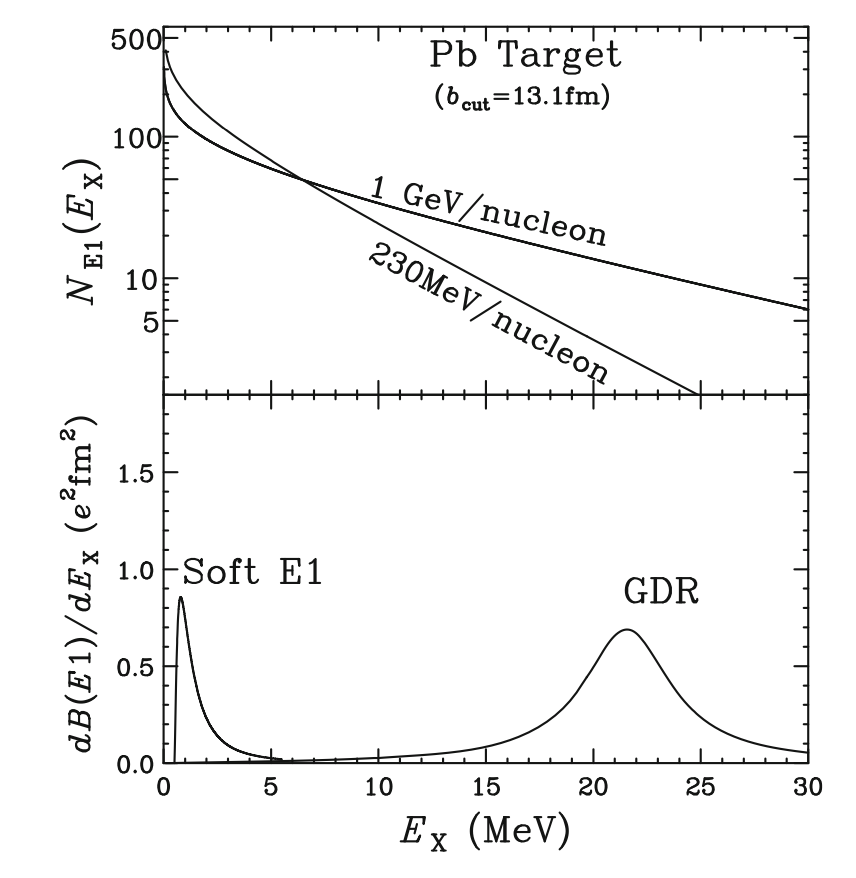
\includegraphics[width=8cm]{chapter2/Virtual_Photon.png}
    \caption[Virtual photon number $N_{E1}(E_x)$ spectra and $dB(E1)/dE_x$ spectrum for halo nucleus\cite{Nakamura23}]{Virtual photon number $N_{E1}(E_x)$ spectra with the $dB(E1)/dE_x$ spectrum for halo nucleus\cite{Nakamura23}. The peak near 1 MeV shows the soft $E1$ excitation, while the peak in high energy region ($\sim 20$ MeV) represents the giant dipole resonance.}
    \label{fig:Virtual_Photon}
\end{figure}

\subsection{Geometry of Two Neutron Halo and Dineutron Correlation}
Another information which can be extracted from $E1$ reduced transition probability is related with the geometrical value of the two neutron halo nucleus. By non-energy weighted cluster sum rule from Esbensen et at. \cite{Esbensen}, the $E1$ reduced transition probability $B(E1)$ in entire energy region can be written as 
\begin{align}
    B(E1) &= \int_{-\infty}^{\infty} \frac{dB(E1)}{dE_x}dE_x \notag \\
        &= \frac{3}{\pi} \bigg(\frac{Z e}{A}\bigg)^2 \langle r^2_{c-nn} \rangle,
        %&= \frac{3}{4 \pi} \bigg(\frac{Z e}{A}\bigg)^2 \langle \vec{r_1}^2 + \vec{r_2}^2 + 2 \vec{r_1} \cdot \vec{r_2} \rangle \notag \\
        %&= \frac{3}{4 \pi} \bigg(\frac{Z e}{A}\bigg)^2 \langle \vec{r_1}^2 + \vec{r_2}^2 + 2\vec{r_1} \vec{r_2} \cos \theta_{nn} \rangle
\end{align}
where $\langle r^2_{c-nn} \rangle$ is a root mean square (rms) distance between the core nucleus and the two center of mass of two neutron. Furthermore, the distance between two neutrons $\langle r^2_{nn} \rangle$ can be obtained from matter radius of halo and core nucleus in the three body model as \cite{Bertulani07}\cite{Hagino07},
\begin{align}
    \langle r^2_{m} \rangle = \frac{A_c}{A} \langle r^2_{m} \rangle_{c} + \frac{2A_c}{A^2} \langle r^2_{c-nn} \rangle + \frac{1}{2A} \langle r^2_{nn} \rangle
\end{align}
where $A$ and $A_c (= A - 2)$ are the mass number of halo and core nucleus respectively. $\langle r^2_{m} \rangle$ and $\langle r^2_{m} \rangle_{c}$ are the matter radius of halo and core nucleus respectively. In this research, for calculation, we use the value $\langle r^2_{m} \rangle = 3.00 (6)$ fm, $\langle r^2_{m} \rangle_c = 2.75 (6)$ fm from the rms radius of $^{17}$B and $^{15}$B respectively \cite{Estrade}. $\langle r^2_{nn} \rangle$ is the distance between two neutrons.
Finally, the opening angle between two neutrons $\langle \theta_{nn} \rangle$ can be obtained as,
\begin{align}
    \cos \frac{\theta_{nn}}{2} = \frac{r_{c-nn}}{\sqrt{r^2_{c-nn} + \frac{r^2_{nn}}{4}} }.
\end{align}


\section{Contribution of Nuclear Breakup}
For evaluating the $B(E1)$ value, we need to extract only the Coulomb dissociation component from the experimental data. In this research, we used $\Gamma$ factor method to remove the contribution of nuclear breakup component from lead target. For extracting the Coulomb dissociation cross section $\sigma(CD)$, we subtract the reaction cross section with the carbon target scaled by $\Gamma$ factor from the one with the lead target. Using this method, we can write the Coulomb dissociation cross section as follows.
\begin{align}
    \sigma_{CD} = \sigma(\text{Pb}) - \Gamma \sigma(\text{C}),\label{eq:CD}
\end{align}
$\sigma(\text{C})$ and $\sigma(\text{Pb})$ are the reaction cross section with carbon and lead target respectively. $\Gamma$ is the ratio of the reaction cross section with lead target to the one with carbon target. The $\Gamma$ factor can be obtained from the geometry between the projectile and target nucleus as,
\begin{align}
    \Gamma_{\text{min}} &= \frac{R_{\text{Pb}} + R_{{}^{17}\text{B}}}{R_{\text{C}} + R_{{}^{17}\text{B}}} = \frac{A_{\text{Pb}}^{1/3} + A_{^{17}\text{B}}^{1/3}}{A_{\text{C}}^{1/3} + A_{^{17}\text{B}}} = 1.75\\
    \Gamma_{\text{max}} &= \frac{R_{\text{Pb}}}{R_{\text{C}}} = \frac{A_{\text{Pb}}^{1/3}}{A_{\text{C}}^{C}} = 2.59
\end{align}
In this experiment, we used $\Gamma = 2.835$ value from calculation including the consideration of incident energy of $^{17}$B at the middle of target (270 MeV/u)\cite{Ogata}.

\section{Invariant Mass Method}
To reconstruct the excited state of ${}^{17}$B at target, invariant mass method is used. Since ${}^{17}$B has no bound excited state and its two neutron separation energy $S_{2n}$ is very small, the dissociation process occurs very quickly. In this case, the invariant mass method is a useful tool to reconstruct the intermediate excited state of the system by measuring the momentum and energy of all of the fragments. The invariant mass of the excited state $M^{*}$ is defined as
\begin{align}
    M^* &= \sqrt{\bigg(\sum_{i} E_i\bigg)^2 - \bigg(\sum_{i}\vec{P}_i \bigg)^2} 
\end{align}
where $E_i$ and $\vec{P}_i$ are the energy and momentum of the fragment $i$ respectively. In this experiment, the excited state of ${}^{17}$B is reconstructed by measuring the momentum and energy of ${}^{15}$B and two neutrons. The relative energy $E_{rel}$ between ${}^{15}$B and two neutron can be written with the invariant mass as
\begin{align}
    E_{rel} &= M({}^{17}\text{B}^*) - (m_{{}^{15}\text{B}} + m_n + m_n)
\end{align}
where $m_{{}^{15}\text{B}}$, $m_n$ and $m_n$ are the mass of ${}^{15}$B and two neutrons respectively. The relative energy $E_{rel}$ is related to the excitation energy $E_x$ of ${}^{17}$B and neutron separation energy $S_{2n}$ as
\begin{align}
    E_{rel} &= E_x - S_{2n}
\end{align}
Figure \ref{fig:Invariant_Mass} shows the schematic representation of the invariant mass method. 

\begin{figure}[t]
    \centering
    \setlength{\unitlength}{1mm}
    \begin{picture}(60,40)
        \put(6,15){$E_x$}
        \put(16,1){${}^{17}$B}
        \put(18,31){$M^*$}
        \put(49,11){${}^{15}$B + n + n}
        \put(29,18){$E_{rel}$}
        \put(33,4){$S_{2n}$}
        %\put(10,0){\dashbox{dash-len}}}
        \thicklines
        \put(10,30){\line(1,0){20}}
        \put(10,0){\line(1,0){20}}
        \put(50,10){\line(1,0){20}}
        \put(20,5){\vector(0,1){24}}
        \put(31,29){\vector(1,-1){18}}
        \thinlines
        \multiput(26,10)(1.2,0){20}{\line(1,0){0.8}}
        \multiput(28,0)(1.2,0){10}{\line(1,0){0.8}}
        \put(28,20){\vector(0,1){10}}
        \put(28,20){\vector(0,-1){10}}
        \put(12,20){\vector(0,1){10}}
        \put(12,20){\vector(0,-1){20}}
        \put(32,5){\vector(0,1){5}}
        \put(32,5){\vector(0,-1){5}}
        
    \end{picture}
    \caption{Schematic representation of the invariant mass method} 
    \label{fig:Invariant_Mass}
\end{figure}